\documentclass[a4paper,10pt]{article}
\usepackage[margin=2mm]{geometry}
\usepackage{tikz}
\usetikzlibrary{calc}
\usepackage{helvet}
\renewcommand{\familydefault}{\sfdefault}
\pagestyle{empty}
\usepackage{pdflscape}

% --- tailles en longueurs TeX ---
\newlength{\cellw}\setlength{\cellw}{1.4cm}
\newlength{\cellh}\setlength{\cellh}{1.2cm}

\definecolor{groupbg}{RGB}{245,248,252}
\definecolor{line}{RGB}{200,210,225}

% \Element{groupe}{periode}{Z}{Sym}{Masse}
% on utilise x=\cellw et y=-\cellh : une unité = 1 cellule (y positive descend)
\newcommand{\Element}[5]{%
	\pgfmathsetmacro{\XX}{#1-1}%
	\pgfmathsetmacro{\YY}{#2-1}%
	\begin{scope}[shift={(\XX,\YY)}]
		\draw[line width=0.25pt,color=line,fill=groupbg,rounded corners=0.8pt]
		(0,0) rectangle (1,1);
		\node[anchor=north west,inner sep=1pt,font=\tiny] at (0,0) {#3};
		\node[anchor=center,font=\bfseries\small] at (0.5,0.45) {#4};
		\node[anchor=south east,inner sep=1pt,font=\scriptsize] at (1,1) {#5};
	\end{scope}%
}

\begin{document}
	\begin{landscape}
		\begin{center}
			{\Large Tableau périodique — Z, symbole, masse molaire}\\[3mm]
			
			% x=\cellw (largeur cellule), y=-\cellh (hauteur cellule : y positif => descend)
			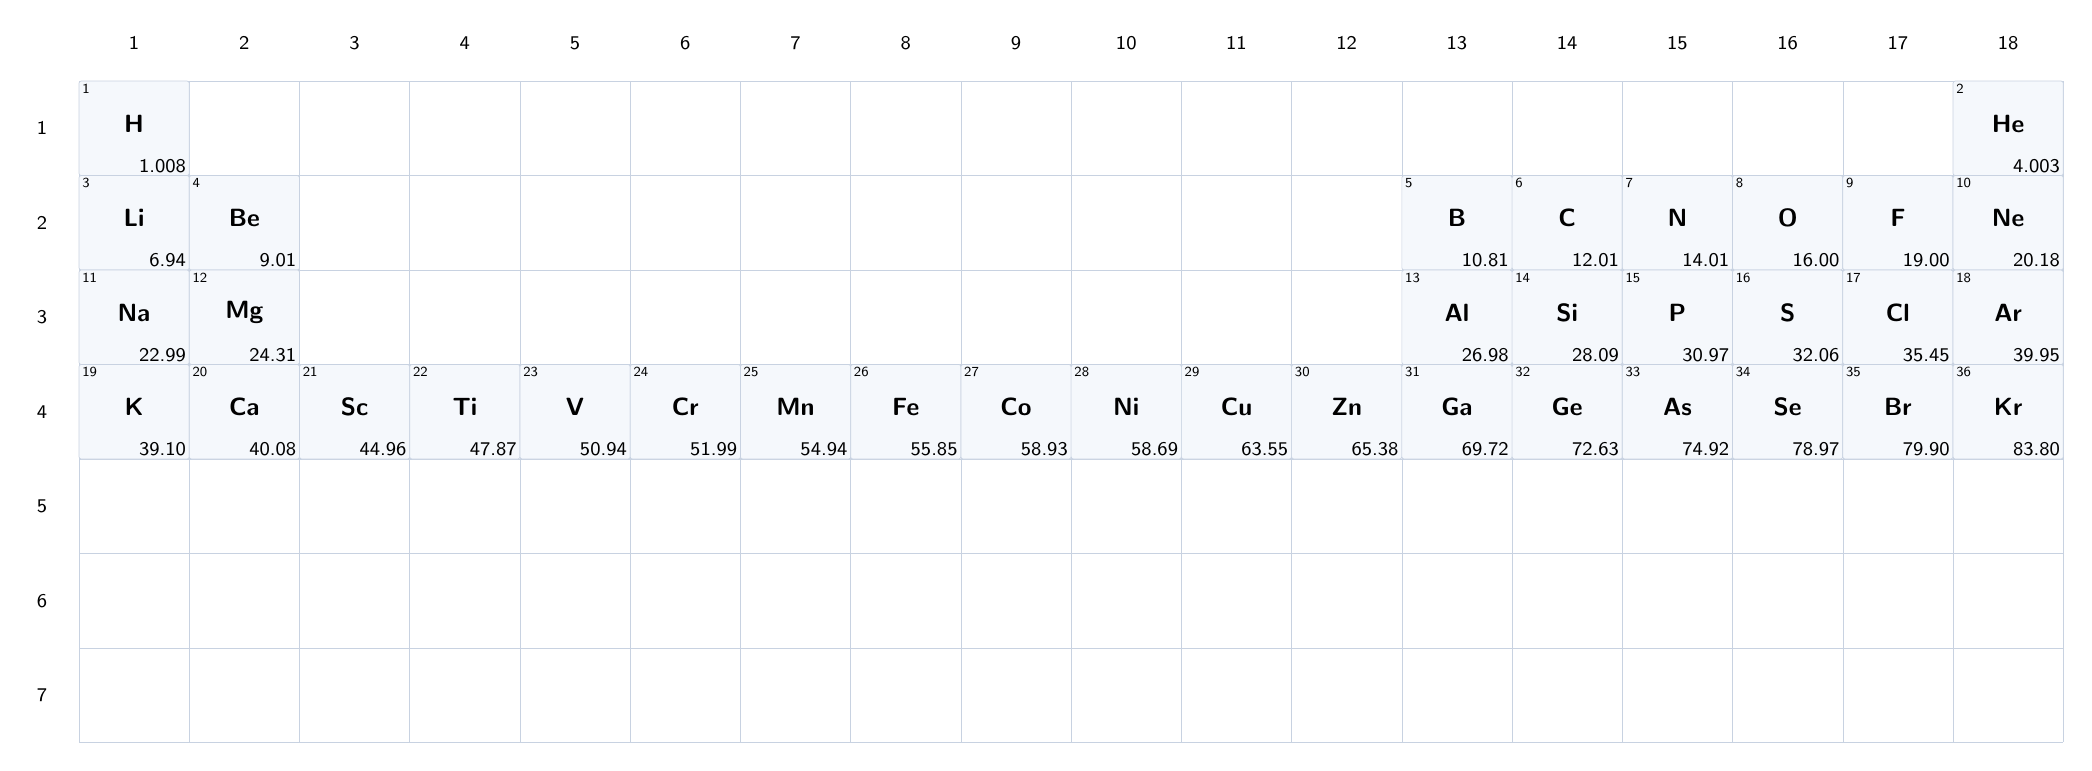
\begin{tikzpicture}[x=\cellw,y=-\cellh]
				
				% grille 18 colonnes × 7 lignes (coordonnées en "cellules")
				\foreach \g in {0,...,18}{
					\draw[line width=0.2pt,color=line] (\g,0) -- (\g,7);
				}
				\foreach \p in {0,...,7}{
					\draw[line width=0.2pt,color=line] (0,\p) -- (18,\p);
				}
				
				% étiquettes de groupes (au-dessus)
				\foreach \g in {1,...,18}{
					\node[font=\scriptsize] at (\g-0.5,-0.4) {\g};
				}
				% étiquettes de périodes (à gauche)
				\foreach \p in {1,...,7}{
					\node[font=\scriptsize,anchor=east] at (-0.2,\p-0.5) {\p};
				}
				
				% --- Exemples (périodes 1 à 4) ---
				\Element{1}{1}{1}{H}{1.008}
				\Element{18}{1}{2}{He}{4.003}
				
				\Element{1}{2}{3}{Li}{6.94}
				\Element{2}{2}{4}{Be}{9.01}
				\Element{13}{2}{5}{B}{10.81}
				\Element{14}{2}{6}{C}{12.01}
				\Element{15}{2}{7}{N}{14.01}
				\Element{16}{2}{8}{O}{16.00}
				\Element{17}{2}{9}{F}{19.00}
				\Element{18}{2}{10}{Ne}{20.18}
				
				\Element{1}{3}{11}{Na}{22.99}
				\Element{2}{3}{12}{Mg}{24.31}
				\Element{13}{3}{13}{Al}{26.98}
				\Element{14}{3}{14}{Si}{28.09}
				\Element{15}{3}{15}{P}{30.97}
				\Element{16}{3}{16}{S}{32.06}
				\Element{17}{3}{17}{Cl}{35.45}
				\Element{18}{3}{18}{Ar}{39.95}
				
				\Element{1}{4}{19}{K}{39.10}
				\Element{2}{4}{20}{Ca}{40.08}
				\Element{3}{4}{21}{Sc}{44.96}
				\Element{4}{4}{22}{Ti}{47.87}
				\Element{5}{4}{23}{V}{50.94}
				\Element{6}{4}{24}{Cr}{51.99}
				\Element{7}{4}{25}{Mn}{54.94}
				\Element{8}{4}{26}{Fe}{55.85}
				\Element{9}{4}{27}{Co}{58.93}
				\Element{10}{4}{28}{Ni}{58.69}
				\Element{11}{4}{29}{Cu}{63.55}
				\Element{12}{4}{30}{Zn}{65.38}
				\Element{13}{4}{31}{Ga}{69.72}
				\Element{14}{4}{32}{Ge}{72.63}
				\Element{15}{4}{33}{As}{74.92}
				\Element{16}{4}{34}{Se}{78.97}
				\Element{17}{4}{35}{Br}{79.90}
				\Element{18}{4}{36}{Kr}{83.80}
				
				% (complète les périodes 5–7 / lanthanoïdes / actinoïdes si tu veux)
				
			\end{tikzpicture}
		\end{center}
	\end{landscape}
\end{document}
